%\subsection{Specific Aim 2: Functional Materials}
\subsection{Specific Aim 2: Hydrodynamics}
\label{subsec:specific_aim_2}
Specific Aim 1 dealt with elastic material properties of self-assembled collections of amphiphiles.
In Specific Aim 2, we include hydrodynamics effects by embedding the particles in a solvent. 
We divide space into the fluid phase and the rigid particle phase.
The fluid phase is modeled by the Stokes equations for an incompressible, zero Reynolds-number fluid. These are coupled to the screened-Laplace equation \eqref{SL}
through viscous and hydrophobic stress balance.
We develope a numerical solver for the mobility problem. 
This leads to simulations of bilayers in external flows where the bilayers are represented by a self-assebled collection of rigid particles.
Finally, we work toward three-dimensional solvers with application in the capillary driven fabrication of micro-materials. 

Hydrodynamic effects are a relevant detail 
because the rates of biological functions like fusion, fission, and pore dynamics rely on viscous dissipation \cite{RYHAM20112929}. 
While hydrophobic attraction causes the particles to self-assemble indepedently of the dissipation mechanism, the trajectories and
equilibrium configurations depend on the fact that the particles travel through a viscous environment. 
Additionally, coarse-grained and molecular dynamics theories include water either explicitly or implicitly in their models. 


\begin{figure}
  \centering{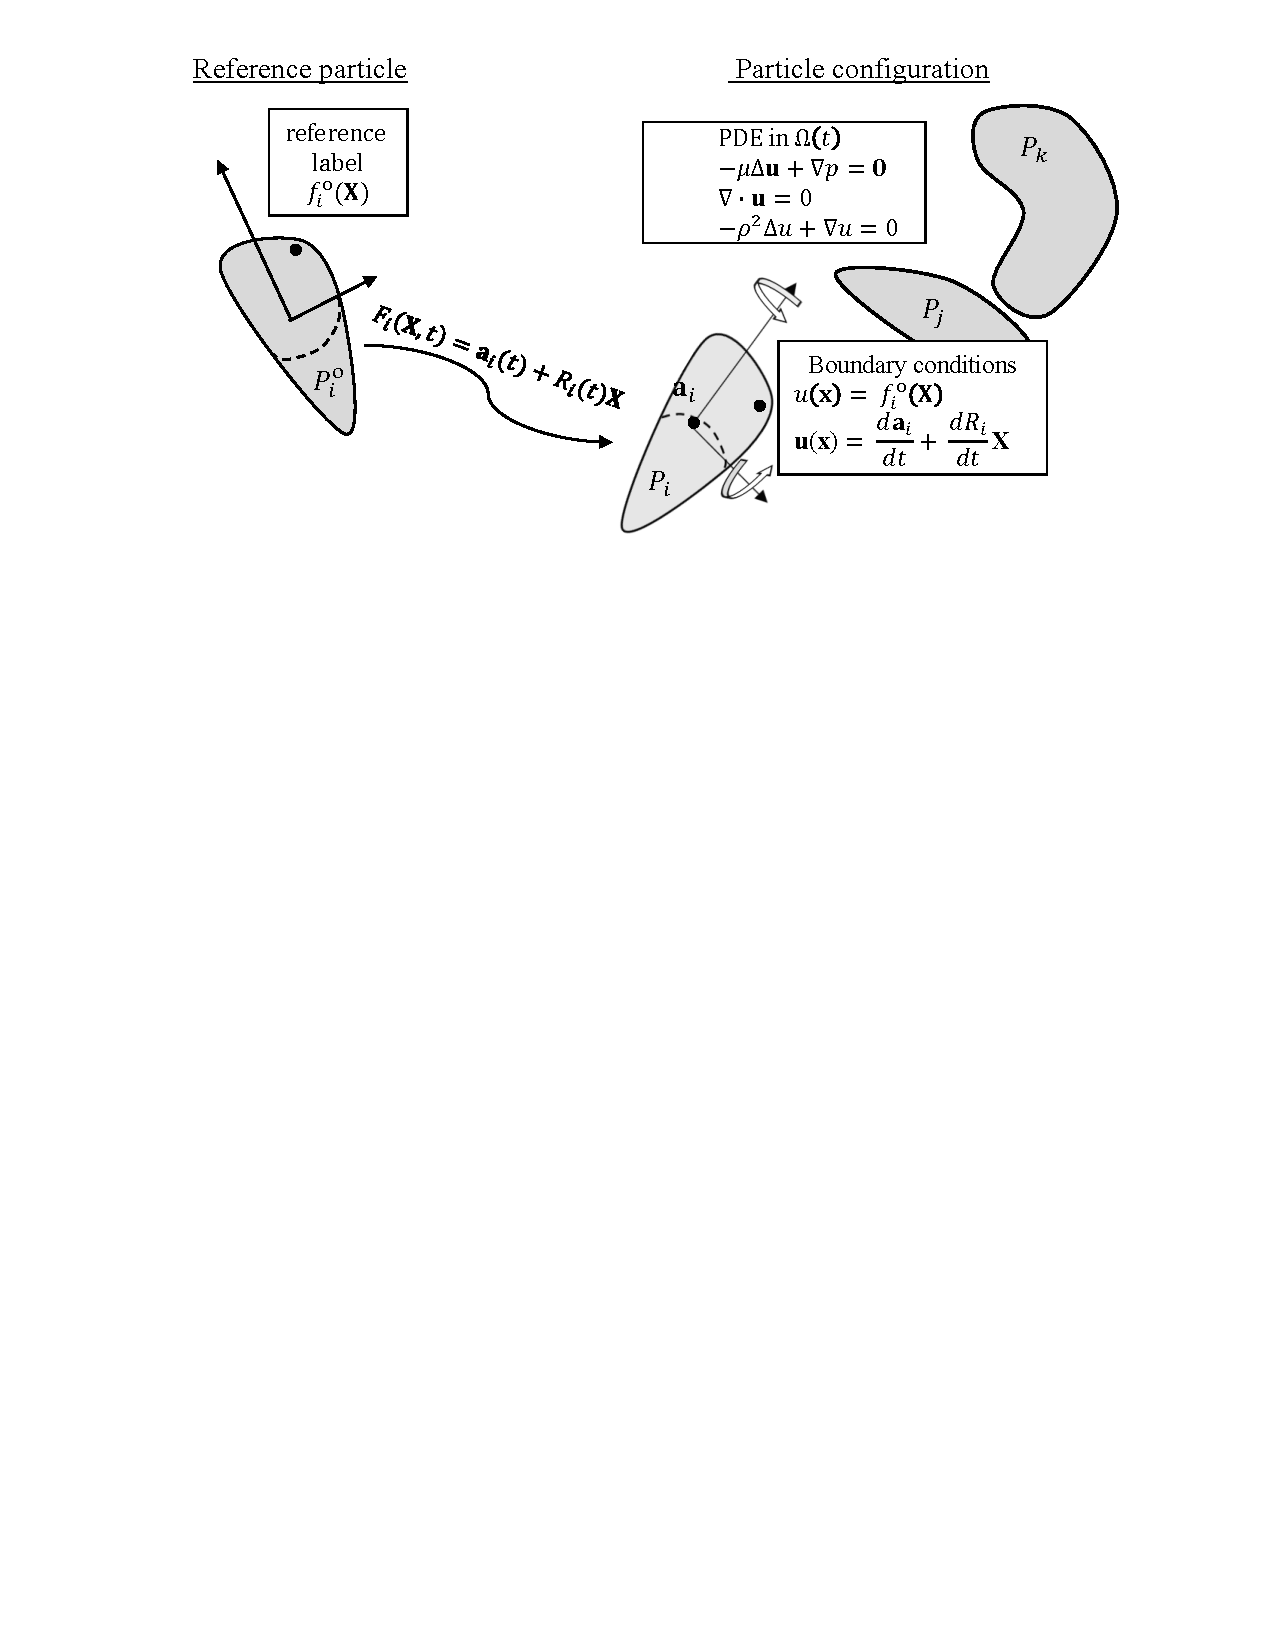
\includegraphics[width=0.8\textwidth]{Figures/domain.pdf}}
    \caption{\label{fig:flow_map}TBD}
\end{figure}
\textbf{Model equations.}
The hydrodynamic interactions enter through the transmission of viscous stresses from one particle to the another.  
We must solve the system 
\setcounter{midequation}{\theequation}
\addtocounter{midequation}{2}

\begin{minipage}[t]{0.44\textwidth}
\begin{subequations}
\begin{alignat}{2}
\label{St1} -& \mu \Delta {\bf u} + \nabla p = {\bf 0}, \\
\label{St2}  & \nabla \cdot {\bf u} = 0,                &&   \text{in } \Omega\\
\label{St3}  & {\bf u }({\bf x}) = {\bf v}_i + {\bf w_i}\times {\bf x}, \;  && \text{for } {\bf x} \in \partial P_i\\
\label{St4}  & ({\bf u } - {\bf u}_{\infty})({\bf x}) \to {\bf 0} && \text{as } {\bf x} \to \infty\\
\notag \\
\tag{\themidequation}
\label{HSB1}  & \int_{\partial P_i} \boldsymbol{\sigma} \boldsymbol{\nu} \,\dif S + {\bf F}_{i} = {\bf 0}\span \span
\end{alignat}
\end{subequations}
\end{minipage}
\addtocounter{equation}{1}
\setcounter{midequation}{\theequation}
\addtocounter{midequation}{2}
\begin{subequations}
\begin{minipage}[t]{0.5\textwidth}
\begin{alignat}{2}
\label{SL1}  - & \rho^2 \Delta u +u = 0, && \text{in } \Omega\\
\label{SL2}   & u({\bf x}) = f_i({\bf x}),\quad  && \text{for } {\bf x} \in \partial P_i\\
\label{SL3} &  u({\bf x}) \to 0 && \text{as } {\bf x} \to \infty \\
\notag \\
\notag \\
\tag{\themidequation}
\label{HSB2}   & \int_{\partial P_i} {\bf x} \times \boldsymbol{\sigma} \boldsymbol{\nu} \,\dif S + {\bf G}_{i} = {\bf 0} \span \span\\
\notag
\end{alignat}
\end{minipage} 
\end{subequations}

\noindent for $i = 1,\dots, N$.
The equations \eqref{St1}--\eqref{HSB2} express a two-way coupling between the flow and bilayer shape.
The particle laden flow changes the shape of the bilayer, and in return the hydrophobic stresses coming
from the altered shape impart a force on the flow. 
The inputs to \eqref{St1}--\eqref{HSB2} are the collection of particle configurations.
Within this system, the activity $u$ solves the screened Laplace equation \eqref{SL1} with the material label boundary condition \eqref{SL2}
and far-field condition \eqref{SL3}. The forces ${\bf F}_i$ and torques ${\bf G}_i$ come from \eqref{totalFG}.
In turn, the fluid velocity ${\bf u}$ solves the Stokes equations (\ref{St1}, \ref{St2}) with background flow boundary condition (\ref{St3}).
The force and torque equations \eqref{HSB1}, \eqref{HSB2} couple the (\ref{St1}--\ref{St4}) to (\ref{SL1}--\ref{SL3}).
The outputs are the collection of velocity and rotation pairs $({\bf v}_i, {\bf w}_i)$ that uniquely satisfy the rigid body boundary condition \eqref{St3}. 

The particle velocity and rotation $({\bf v}_i, {\bf w}_i)$ update the particle configurations:
\begin{alignat}{3}
\label{Hupdate1}   \frac{\dif {\bf a}_i}{\dif t} = {\bf v}_i,      \quad  \frac{\dif {\bf R}_i}{\dif t}  = A({\bf w}_i),\quad i = 1, \dots, N.
\end{alignat}
Recall that $A({\bf w}_i)$ is the skew-symmetric matrix with axial vector ${\bf w}_i$.
Also, ${\bf a}_i$ is the particle center the rotation matrix ${\bf R}_i$ defines the orientation.
That way, the particle configurations come from the flow maps $F_i({\bf x},t) = {\bf a}_i(t) + {\bf R_i}(t){\bf x}$ with
$P_i(t) = F_i(P_{0i},t)$ and $f_i(F_i({\bf x},t)) = f_{i0}({\bf x})$ where $P_{i0}$ and $f_{i0}$ are the $i$th reference particle
and material label respectively.
When there is no background flow ${\bf u}_{\infty} = {\bf 0}$, the system obeys the energy law
$\frac{\dif}{\dif t} \Phi + \int_{\Omega(t)} \mu |\nabla {\bf u} + \nabla {\bf u}^T|^2 \,dx = 0,$ 
and the particle configurations tend toward a local equilibrium.

Numerically solving \eqref{St1}--\eqref{HSB2} is a nontrivial matter.
The principle challenges are \textbf{(1)} the domain $\Omega(t)$ and boundary conditions $f_i$ are constantly changing
with changes in the particle configuration \textbf{(2)} a high degree of spatial accuracy is required to resolve the fields 
between adjacent particles and \textbf{(3)} the computational complexity grows with the number of particles. 
Specific Aim 3 describes how we address these challenges. 

\textbf{Simulation studies.}
We simulate two-dimensional vesicle bilayers in external flows using \eqref{St1}--\eqref{HSB2}.
The vesicle bilayer is formed by a many-body collection of amphiphilic particles.
At large length scales and for large particle-number, the bilayer behaves as an elastic membrane,
in two-dimensions an elastic curve. 
This will lead to a deeper understanding of the elastic properties established by Specific Aim 2.

We consider two kinds of external flows: shear flow and extensional flow. 
Specifically, we deal with the background flow using the representation 
\begin{equation}
\label{PowerMiranda}
{\bf u} = {\bf u}_{\infty} + D\eta + \sum_{i=1}^N S(\cdot, {\bf a}_i) {\bf F}_i + R(\cdot, {\bf a}_i) {\bf G}_i.
\end{equation}
where $S(\cdot, {\bf a}_i)$ and $ R(\cdot, {\bf a}_i)$ are stokeslets and rotlets supported at the particle centers ${\bf a}_i.$
The symbol $D$ denotes the Stokes double layer integral operator (see Specific Aim 3).   
The representation \eqref{PowerMiranda} automatically satisfies \eqref{St1}, \eqref{St2}, \eqref{St4} and \eqref{HSB1}.
We solve for the unknown density $\eta : \partial \Omega \to \mathbb{R}$ by requiring that jump in viscous stress
vanished across $\partial P_i$. This jump condition guarantees that ${\bf u}$ is a rigid motion within each particle,
and by continuity, equals a rigid motion on the particle boundary as required by \eqref{St3}.

We will compare the behavior of our particle-based vesicles in Stokes flow to well-established results.
To test area incompressibility, we form the bilayer midplane by fitting to the particle centers. Under moderate shear rates,
the vesicle elongates and takes on an elliptical shape. We will study the increase in midplane area as a function of shear rate.
Additionally, we will test for tangential divergence of velocity.
Researchers have devised to model area incompressible and
volume conserving membranes
\cite{torres-sanchez_millan_arroyo_2019, mahapatra_saintillan_rangamani_2020, Steigmann99, C6SM02452A}.
Our preliminary results show that the particle-based bilayers have the same area modulus, about 60 \kBT,  as that of real lipid bilayer membranes,
and so we expect realistic results from our flow simulations with regard to area incompressibility.  It is noteworthy that
area incompressibility is some sense baked into the model through the hydrophobic attraction. 

Bilayer membranes have a small permeability to water \cite{323e9a2f0c58487ea82518d7a1f96485},
and so modelers often assume a vesicle membrane that conserves volume. In our particle-based approach, water motion across
the bilayer is limited by the size of the gaps between the particles, which is an artifact of coarse-graining.
Making these gaps smaller comes at the expense of numerical accuracy, and so we will assess if there is a reasonable trade-off
between approximate volume conservation and simulation complexity. 

\begin{wrapfigure}[16]{r}{0.32\textwidth}
\centerline{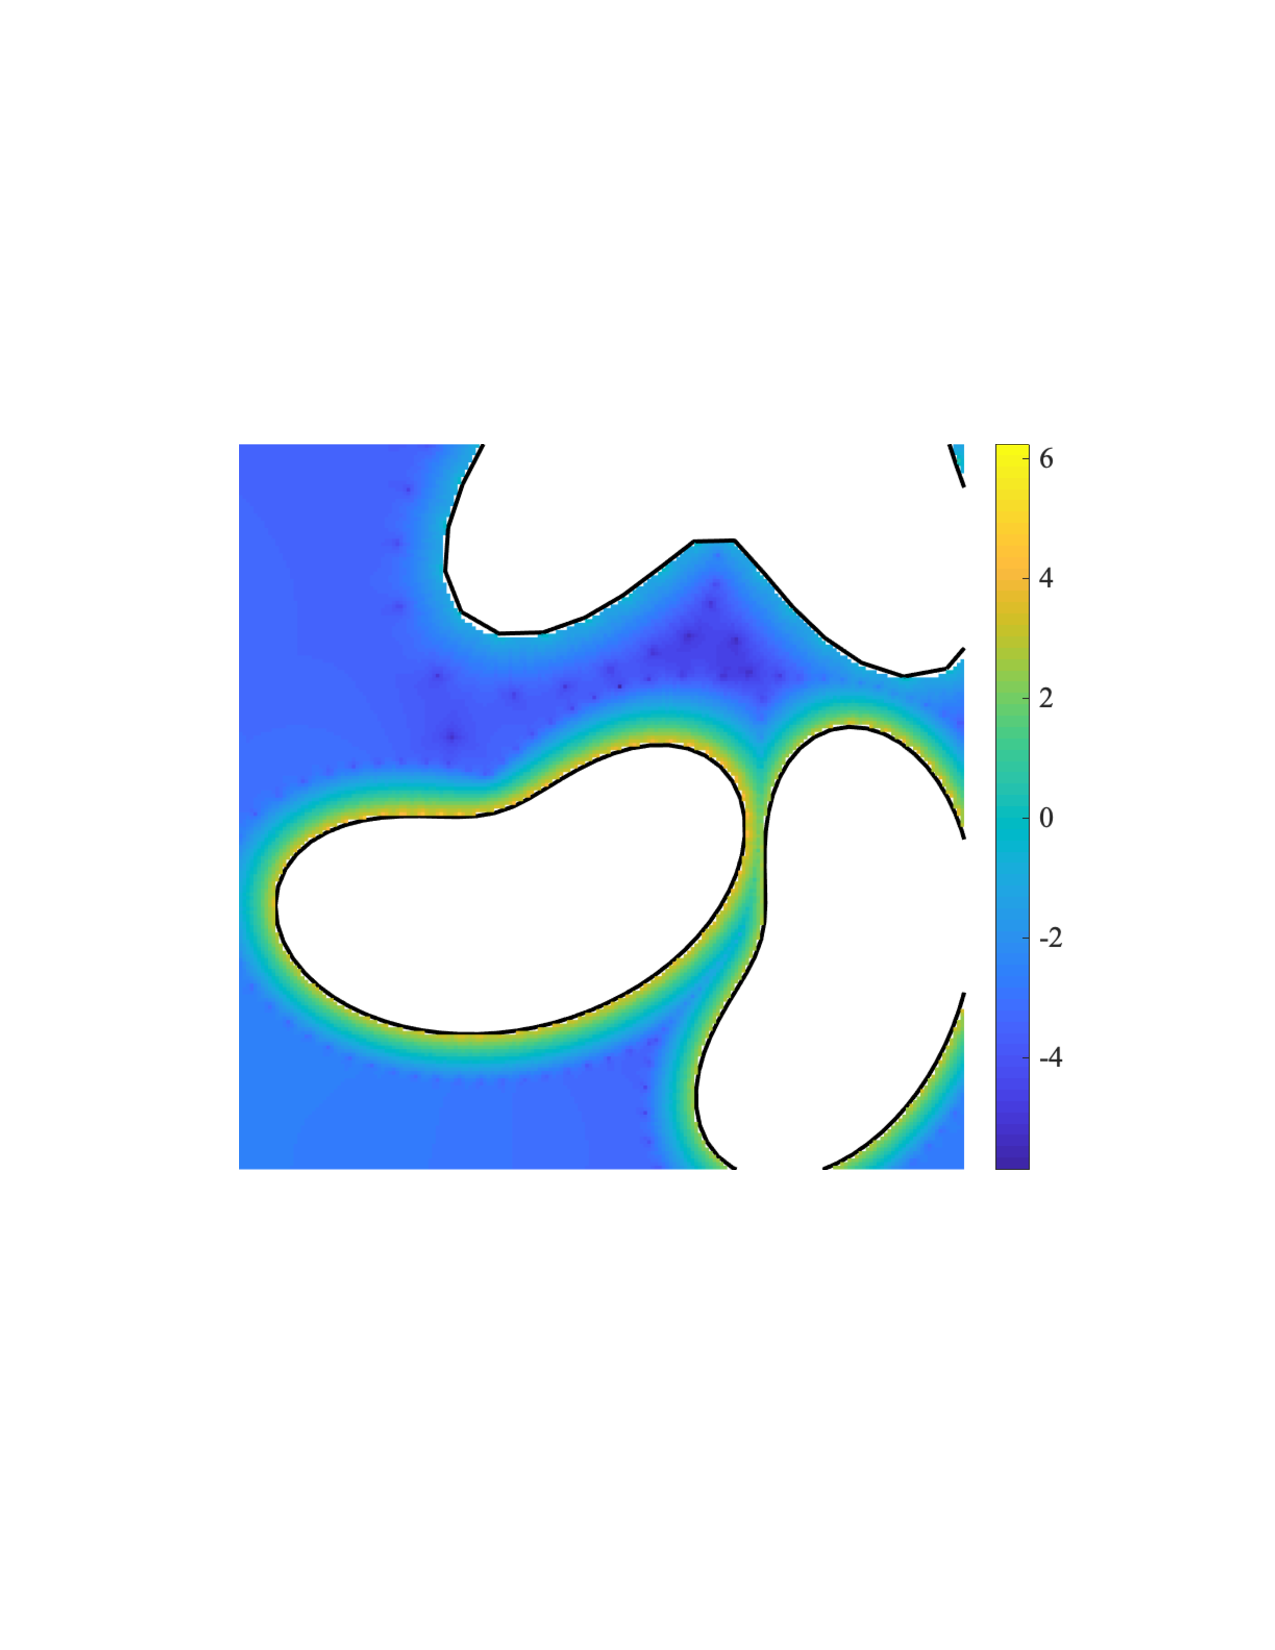
\includegraphics[width=0.32\textwidth]{figures/BIError.pdf}}
\caption{
\label{fig:bierror}  
  Gradient error between an exact and boundary integral solution of \eqref{SL}.
}
\end{wrapfigure}
Finally, the particle-based vesicle bilayers have two distinct leaflets.
The inner and outer leaflets consists of the particles in contact with the vesicle interior and 
surrounding fluid respectively. Since there the separation between these layers is roughly fixed,
about 2 nm, certain fluid mechanical effects arise that are not present in zero-thickness membrane models. 
An important effects we observe is that the leaflets slide against one another under shear flow. 
This implies that part of the viscous dissipation in the aqueous phase is enhanced by intermonolayer friction
\cite{SHKULIPA2005823, ShkulipaThesis}. We will characterize the intermonolayer
slip as a function of shear rate, vesicle diameter and particle geometry. 

\textbf{Novel reciprocal relations.}
We prove a, to our knowledge new, result concerning the evaluation of Maxwell-type stresses. 
\begin{proposition}
  \label{prop:recip}
  Suppose that $u = \sum_{i=1}^N u_i$ where $u_i$ is a solution of the screened Laplace equation
  in $\mathbb{R}^3 \setminus P_i$ for $i=1,\dots, N.$ Then 
  \begin{equation}
    \label{eq:reciprocal}
{\bf F}_i = \sum_{j \neq i} \int_{\partial P_i}[\boldsymbol{\sigma}_{ij} + \boldsymbol{\sigma}_{ji}]\boldsymbol{\nu}\,\dif S,\quad
{\bf G}_i = \sum_{j \neq i} \int_{\partial P_i} {\bf x} \times [\boldsymbol{\sigma}_{ij} + \boldsymbol{\sigma}_{ji}]\boldsymbol{\nu}\,\dif S, \quad i = 1\dots, N.
\end{equation}
where $\boldsymbol{\sigma}_{ij} = \rho^{-1} u_iu_j {\bf I} + \rho(\nabla u_i \cdot \nabla u_j {\bf I} - 2 \nabla u_i \otimes \nabla u_j)$ and
$[\cdot]$ denotes the jump in stress across $\partial \Omega.$ 
\end{proposition}
As described in Specific Aim 3, we solve \eqref{SL1}--\eqref{SL3}  using a double layer potential representation.
This representation involves a strongly singular integral, and without the aid of specilized
quadrature routines, leads to large numerical errors when evaluating the the hydrophobic stress \eqref{stress} along the particle boundaries (see Figure \cite{fig:bierror}).
The identity in Proposition \ref{prop:recip} gets around this critical issue by utilizing the fact that $u_j$, $j\neq i$ is smooth and the normal derivative
of  $u_i$ continuous across $\partial P_i$. Despite the large gradient errors in Figure \ref{fig:bierror}, the force and torque
calculated by \eqref{eq:reciprocal} achieved $10^{-4}$ accuracy.

Additionally, hydrodynamics interactions are also relevant the fabrication of complex microscopic three-dimensional structures \cite{Cho2010}.
Over the past decade, there has been an explosion of interest in small-scale processes that utilize capillary forces dominate,  van der Waals interactions and thermal noise  \cite{Zhang2017}, to coordinated movement and bind  material subunits. Two prominent fabrication techniques are capillary origami 
\cite{Pandey2011,Leong2007,Reynolds2019} and colloidal self-assembly \cite{Dasgupta2017,Siontorou2017}. Capillary origami uses principles of elastocapilirity wherein elastic solids deform under surface tension \cite{Bico2018,VanHonschoten2010}. In self-assembly of colloids, 
particles exhibit similar thermodynamic behavior of molecular systems, except that the behavior occurs over observable, long time scales \cite{Zhang2017}. 
and can determine which local equilibria the system tends towards.


